\chapter{Recommender System} \label{chap:Recommender}

This chapter will discuss the machine learning approach to building a Recommender system proposed in \autoref{sec:RecSystems}. It discusses the different approaches to creating this Recommender system and explains the reasons behind the chosen method.

\section{Information Gathering}
The Recommender System requires a representation of a users preferences in a format suitable for statistical analysis. To generate this representation, we need to collect some form of feedback from the users. There are three types of feedback that can be retrieved from the user.

\subsubsection{Implicit Feedback}
The user preferences are obtained automatically from implicit user actions on the system. This reduces the amount of work and input needed by the user, however it is less accurate. Implicit data we can collect is the number of times a user clicks on a trail, but a user clicking on a trail does not reflect their feelings towards that trail.

\subsubsection{Explicit Feedback}
The system requires users to reflect on the choices of trails that they make. In our system we provide a review system discussed in \autoref{subsec:trailDescription}, that asks users to rate the trails that they've run \cite{jawaheer2010comparison}. As the users provides this data explicitly, it is more accurate and more greatly reflects the users preferences. However, users are less likely to leave reviews and ratings unless forced too.

\subsubsection{Hybrid Feedback}
A combination of both Implicit and Explicit feed-backs, using the strengths of both and minimising the weakness of each feedback method. 

Due to the inaccuracy of implicit feedback, especially in our scenario, I decided to just rely on explicit feedback.

\section{Choosing A Recommender Algorithms} \label{chooseRecAlg}
There are multiple different ways of implementing Recommender system. For a machine learning approach, there are three popular approaches used which are
\begin{itemize}
    \item Content-based filtering
    \item Collaborative filtering
    \item Hybrid Technique
\end{itemize}
as shown in figure \ref{fig:recommenderSystemTypes}. The main feature that the approaches listed above is similarity.

\begin{figure}[htb!]
    \centering
    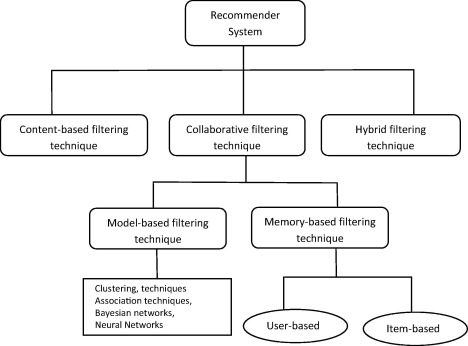
\includegraphics[width=0.5\textwidth]{recommenderSystemTypes.jpg}
    \caption{Types of Recommender Systems \cite{isinkaye2015recommendation}}
    \label{fig:recommenderSystemTypes}
\end{figure}

\subsubsection{Content-based filtering}
\acrfull{cbf} recommends items based on information known about the particular item \cite{pazzani2007content}. The system would have some meta-data about the item, for example, in our scenario we would have extra information about trails such as the type of terrain, location, elevation etc. Items are recommended to the user based on features extracted from users history of positively rated items that represents a users preferences \cite{isinkaye2015recommendation}.

\acrshort{cbf} resolves some of the problems of \acrshort{cf}. The system can still recommend items to users who have not rated any items \cite{burke2002hybrid}. However the the strength of the system greatly relies on how well the content analysis is. 

Content Analysis is the technique of mapping symbolic data into data in a matrix format suitable for analysis \cite{roberts2001content}. For some domains such as news and publications it is quite effective, but for user data that is quite subjective and can be influenced by a large number of variables, it can be difficult and the attributes retrieved may not be suitable to categorise a trail. Having the user add attributes to trails is not a very user friendly method as users are not inclined to perform such menial tasks.
 \ref{fig:contentBasedFiltering}
\begin{figure}[htb!]
    \centering
    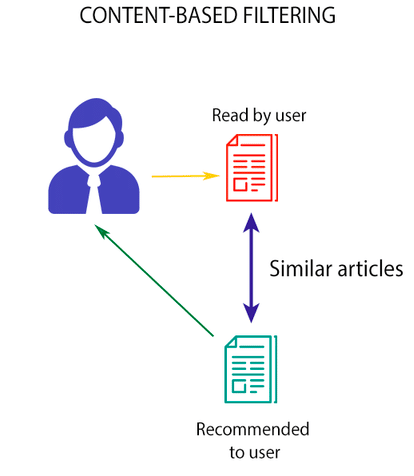
\includegraphics[width=0.5\textwidth]{content-based-filtering.png}
    \caption{Content-based filtering \cite{contentFiltering}}
    \label{fig:contentBasedFiltering}
\end{figure}

\subsubsection{Collaborative filtering}
\acrfull{cf} is a domain independent technique especially useful when content analysis of the items cannot be easily done \cite{isinkaye2015recommendation}. It does so by matching users that are similar based on the user preferences and using this matching to make recommendations \cite{herlocker2004evaluating}. The idea is that, user A likes routes 1 \& 2 and user B likes routes 2 \& 3. As user A and user B like the same route (route 2), then they are similar and user A would also like route 3. 

This property can be seen in real life and works extremely well. People are more likely to trust the suggestions of their friends, i.e. people that they are the most similar with. With this system, you do not need to know any extra information on the routes you are running the algorithm on. We us either explicit information such as user ratings, or implicit information such as number of views on a route, to determine the routes users like. Example shown in figure \ref{fig:collaborativeFiltering}.

\begin{figure}[htb!]
    \centering
    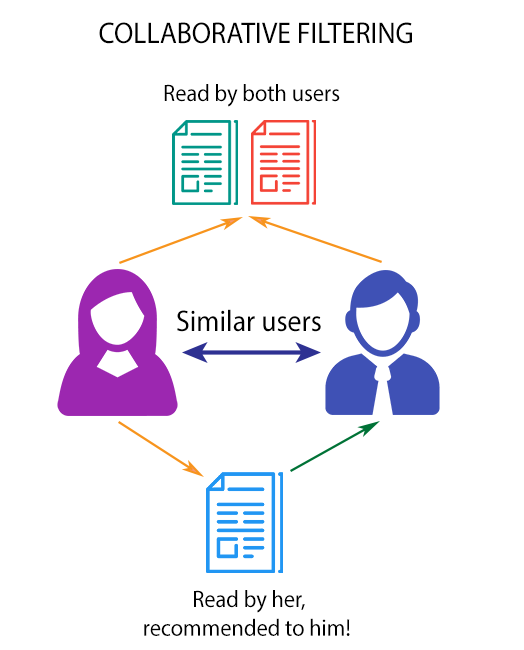
\includegraphics[width=0.5\textwidth]{collaborative-filtering.png}
    \caption{Collaborative filtering \cite{collabFiltering}}
    \label{fig:collaborativeFiltering}
\end{figure}

As trails are quite hard item to perform content analysis on, I decided to chose the collaborative filtering technique. It is best suited to trail running as users are more likely to run routes recommended to them by others.

\subsubsection{Hybrid Recommender Systems}
Hybrid Recommender systems simply combine the results of both collaborative and content-based techniques \cite{claypool1999combing}. The results from both the system's would then have to be ranked again in the combiner as shown in figure \ref{fig:hybridRecommenderSystems}

\begin{figure}[htb!]
    \centering
    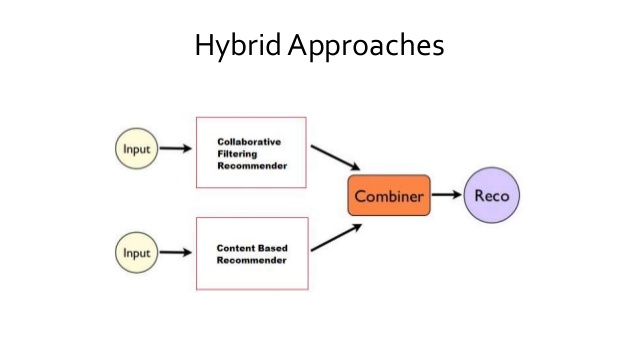
\includegraphics[width=0.5\textwidth]{hybrid-approaches.jpg}
    \caption{Hybrid Approaches \cite{hybridrecommender}}
    \label{fig:hybridRecommenderSystems}
\end{figure}

Although this may be a more appropriate approach to building Recommender Systems, it still requires the complexities from content-based filtering, hence this approach was not used. For this reason, we use a \acrlong{cf} Technique.

\section{Collaborative Filtering}
Collaborative filtering techniques require the system to find users that are similar based on their user preferences inferred from the ratings they give trails they have run previously. There are 2 main approaches to collaborative filtering. We compare these methods below to decide which method is is best suited to our application.

\subsubsection{Memory based Technique}
Memory based based techniques calculate a similarity scores between users or between trails based on the ratings users give trails  \cite{wang2006unifying}. It uses statistical calculations such as the Pearson Correlation Coefficient \cite{benesty2009pearson}, or the Cosine Similarity \cite{michie1994machine}, to calculate the similarity which is weighted against the ratings provided to recommend and rank trails to new users.

This method struggles with performance as the calculations have to be calculated for each individual user on every request. This creates a bottleneck, slowing down the system to perform these calculations. It also means that the system is not very scalable, as users grow, the system will slow down even more. Another issues is the system cannot adjust to user changes quickly. The lack of a model being trained means the system cannot adjust to changes in user preferences.

\begin{figure}[htb!]
    \centering
    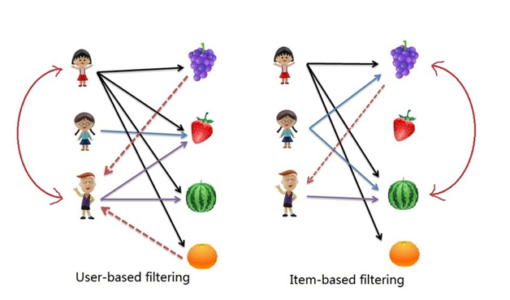
\includegraphics[width=\textwidth]{collab-filtering-types.png}
    \caption{Memory based techniques to collaborative filtering \cite{collabFilteringTypes}}
    \label{fig:collabFilteringTypes}
\end{figure}

\subsubsection{Model based techniques}
To improve on the issues of the memory based techniques, we can use model based techniques. We create a machine learning model that will be trained on a data set of user-trails ratings using the Matrix Factorisation method described in section \ref{matrixFactorization}. We will use a neural network described in section \ref{neuralNetwork}

\section{Matrix Factorisation} \label{matrixFactorization}
To be able to predict trails that would be most suitable to a user, the system needs to learn two main features about the users and trails:
\begin{itemize}
    \item what features a specific user likes in trails
    \item what features a route has that users like
\end{itemize}
We can learn these features using a method called Matrix Factorisation, which is one of the top methods proposed during the Netflix Prize \cite{bell2007lessons}.

We can convert our user-trails ratings from our database into a user-trail matrix. Matrix Factorisation is the process of decomposing a user-trail rating matrix into a product of 2 lower dimension rectangular matrices \cite{koren2009bellkor} as shown in figure \ref{fig:matrixFactorization}.

\begin{figure}[ht]
    \centering
    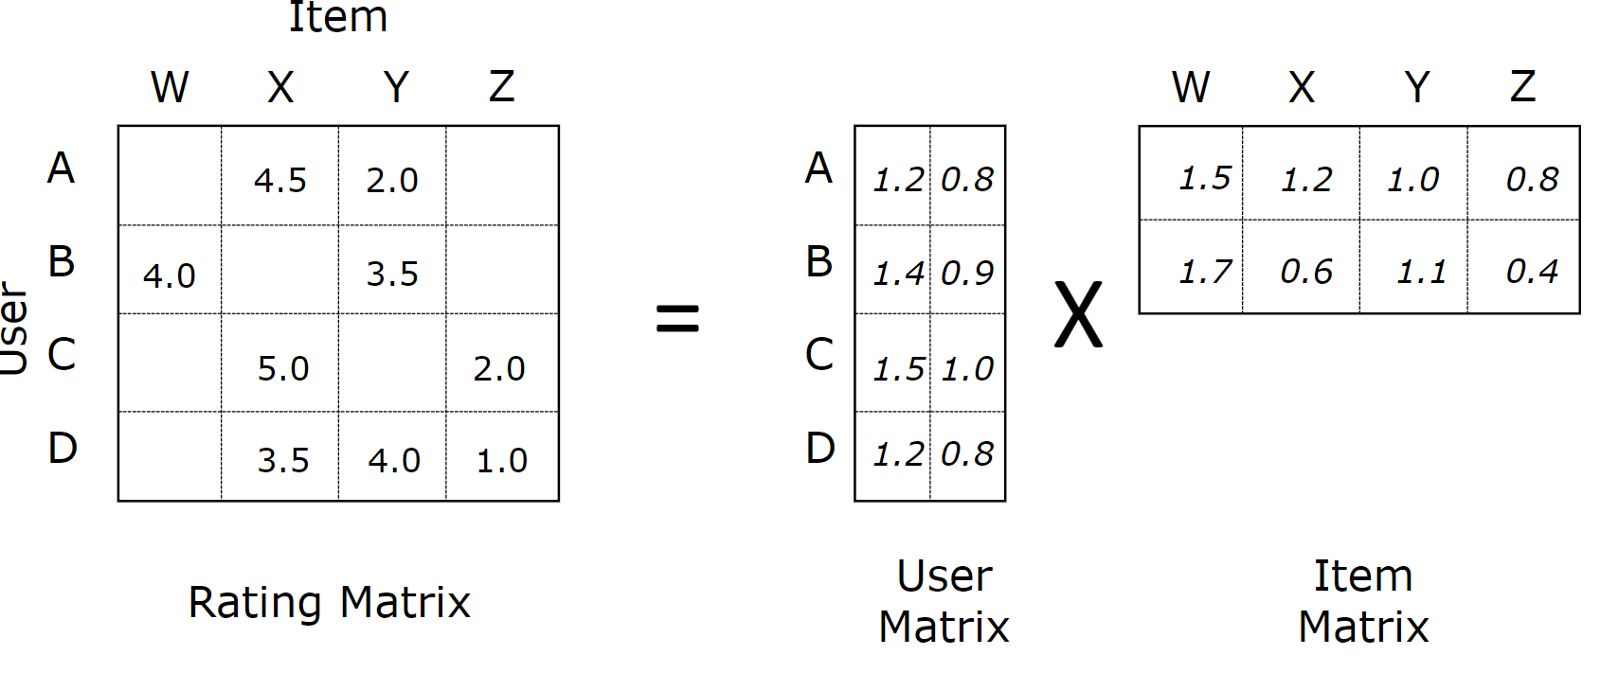
\includegraphics[width=\textwidth]{matrix-factorization.png}
    \caption{Example of Matrix Factorisation}
    \label{fig:matrixFactorization}
\end{figure}

We can represent the above mathematically as 
\begin{equation}
    R \approx P \times Q^T
\end{equation}

Where $R$ is our ratings matrix of size $i \times j$, where $i$ is the number of users and $j$ is the number of trails. $P$ is a user-feature matrix of size $i \times k$ where $k$ is the number of features. $Q$ is a trail-feature matrix of size $u \times k$ and $Q^T$ is its transposition.

As the lower dimension matrices are a decomposition of the ratings matrix, they represent the factors that users use to decide their ratings. Our goal is to find the values for these lower dimension matrices that best describe the ratings matrix and hence best describe the users and trails. These matrices in essence become our user preferences and trail attributes.

These features are also known as \Gls{latent} features because, we do not know explicitly what the features are or even if they exist. The values in the feature matrices could represent the terrain of a trail, or the pollution around the trail, or any feature, however, without rigorous analysis of these values, we can not draw any conclusions as to what they mean.

This does mean that we do not really know the reasons why users like certain trails and we cannot share that back to the user or use that in any other analytic methods. However, this does not in anyway affect the accuracy of the Recommender system. 

To optimise the values in our lower dimension algorithms, we need to calculate how wrong our initial predictions are from our initial matrices. We calculate this loss value using a Loss function. This is then used to update our matrices towards their optimal value using Gradient Descent.



\subsection{Learning Process}
Our initial lower dimensional matrices are initialised to random values. The learning process is to optimise the values of the lower dimension matrices such that the predicted values calculated for ratings are close to the original matrix ratings values. Hence for each $r_{ij} \in R$ we want to calculate $\hat{r_{ij}}$:

\begin{equation}
    \hat{r_{ij}} = p_i \times q_j^T = \sum_{k=1}^{k}{p_{ik}q_{jk}}
\end{equation}

To optimise this we first need to calculate our loss value. This indicates how far away from the actual value our predicted value is

\subsubsection{Loss Function}
A loss function\footnote{also known as a cost function} is a statistical mapping of the correctness of an event or value \cite{wald1950statistical}. Loss functions are a big part of machine learning models as they allow us to empirically evaluate a the model as discussed in \autoref{subsec:evaluationMetrics}. They are also used to train the models, used in the learning phase to discover how our values need to be optimised. 

Choosing a loss function depends on the type of problem you wish to solve and also require a lot of experimentation. From \autoref{subsec:mlApproach}, we know that our Recommender systems can be categorised as a Regression Analysis for regression problems. The loss function we use is called the \acrfull{mse}.

The mean squared error is the measure of an average of the square differences between the predicted values of and the actual values.

\begin{equation} \label{eqn:mseLossFunction}
    MSE = \frac{1}{N}\sum_{i=1}^{N}{({p_i}-{a_i})}^2 
\end{equation}

Where $N$ is the number of iterations performed when training our model. $p_i$ is our predicted value for the $ith$ iteration and $a_i$ is the actual value. Squaring this value has two benefits. It makes the value absolute, as we only care about the difference and not the sign. It also ensures that our loss van be modelled as a quadratic functions. This benefits the system as it ensures there is only one minimum value, (one optimised value). This gives the allows us to easily know when the system has reached the best optimisation possible without over-shooting the minimum.

\subsubsection{Gradient Descent}
Gradient descent is an optimisation algorithm that aims to minimise a loss function by repeatedly taking descent learning steps over a negative gradient towards a minimum value. The gradient descent algorithm takes in a learning rate. This tells us the size of the learning steps we take. 

\begin{figure}[ht]
    \centering
    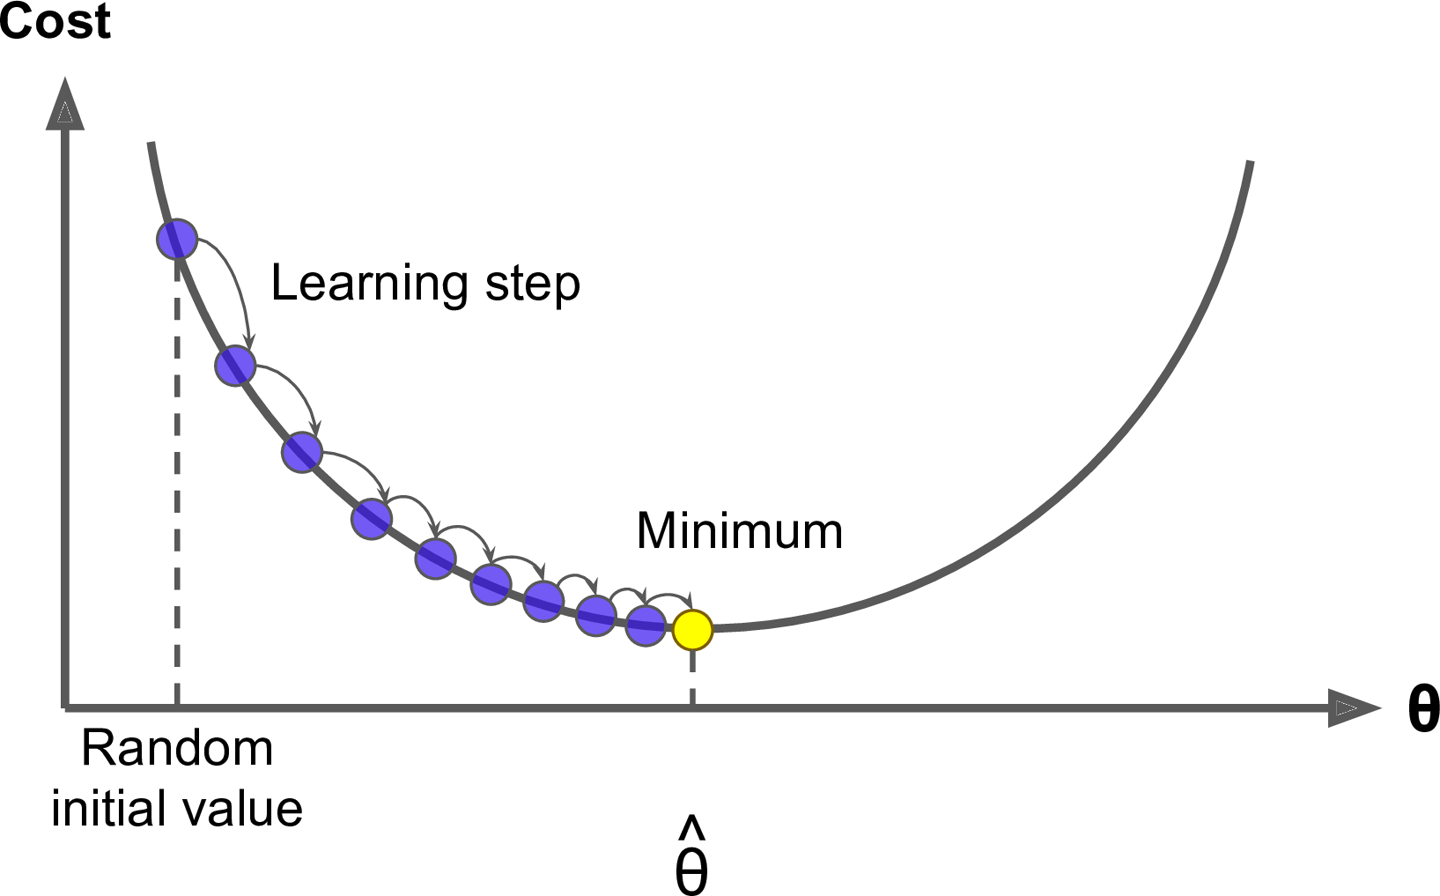
\includegraphics[width=0.75\textwidth]{gradient-descent.png}
    \caption{Gradient Descent \cite{gradientDescent}}
    \label{fig:gradientDescent}
\end{figure}

The gradient descent algorithm used is called \acrfull{adam} which is a variant of \acrfull{sgd}. In gradient descent, we train our model in batches, the number of samples used to train the model during a single iteration. \acrshort{sgd} is a way of performing large-scale machine learning with large data sets and sample sizes \cite{bottou2010large}. It does so by randomly shuffling the sample size and using one sample size per iteration, using the result of that to estimate the others. This generally means that it's more noisy and we need smaller learning steps, but it does not affect the learning process and reduces computation need.

\acrshort{adam} is based on adaptive estimates and lower-order momentum first published in 2014 \cite{kingma2014adam}. It is a complex technique that even further increases the speed of training.

\subsection{Improving with Bias}
To improve our model, we can introduce bias. In real life, you would trust a user that has run more trails than a user that has run fewer routes. This also applies for routes that have been run by more users. We can include this feature into our model to help improve the model created by adding bias values related to each user and each item (route). We include this bias in when training our model. Our new predicted ratings $\hat{r_{ij}}$ can be calculated as

\begin{equation}
    \hat{r_{ij}} = b_i + b_j + {q^{T}_{j}}{p_i}
\end{equation}

Where $b_i$ is our user bias and $b_j$ is our trail bias.

\section{A Deep Learning Approach} \label{neuralNetwork}
Deep learning is a category of machine learning that based on Artificial Neural Networks. Neural networks is a framework for modelling solutions to common machine learning problems based on the brains biological networks \cite{van2018artificial}. 

Neural networks consist of:
\begin{itemize}
    \item An input layer which has our initial input values.
    \item One or more hidden layer that take in as inputs, the values of the nodes from the previous layer and a weight the represents the strength between the current node and the previous node. Each node in this layer uses an activation function to output a value.
    \item An output layer, which will have our final predictions.
\end{itemize}

\begin{figure}[ht]
    \centering
    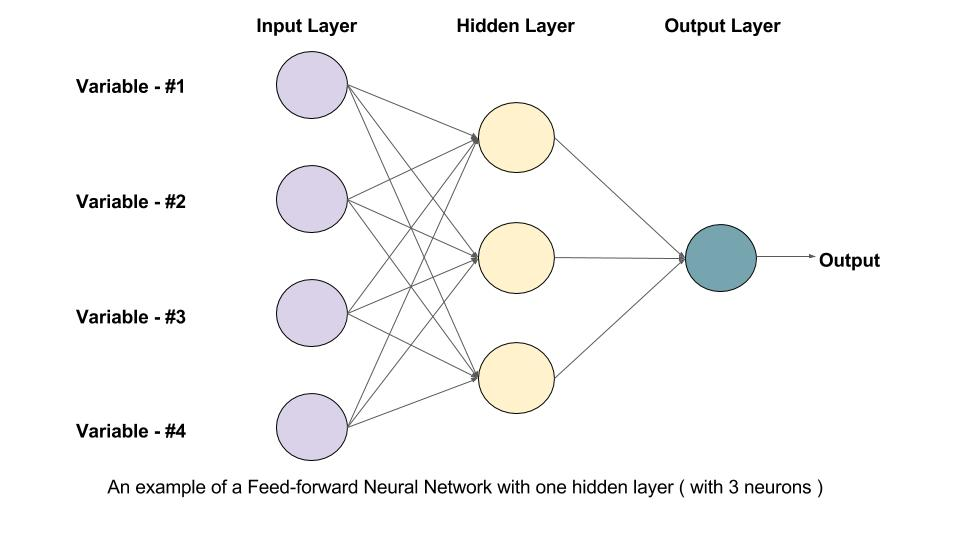
\includegraphics[width=0.7\textwidth]{neural-net-example.jpg}
    \caption{Neural Network Example \cite{neuralNet}}
    \label{fig:neuralNetworkExample}
\end{figure}


We can create our model discussed in section \ref{matrixFactorization}, using a neural network, making the model more robust. The user and and items feature matrices are flattened and concatenated to form our input layer. Then a fully connected hidden layer, that is each node in the hidden layer is connected to every node of the input layer. The hidden layer uses a ReLU activation function \cite{li2017convergence}. Lastly, an output layer with one node that we use to calculate our loss function. Each node also have a bias value that is added in the activation function calculation. The approach used hear was based of a lecture from Jeremy Howard \cite{jeremy2016deep}.

\subsection{Preventing over-fitting}
One of the main problems with machine learning approaches is over-fitting and under fitting.

\paragraph{Under-fitting} is a problem that occurs when the model does not fit the data it's trained on. This happens when not enough iterations has been performed during training making our loss function value worse.

\paragraph{Over-fitting} is when our model is trained to match to perfectly with our training data-set and therefore has a hard time to predict when we have a completely new data. To prevent this in Neural Networks we can add a dropout layer to the neural network. Drop out layers kill random nodes in our neural network during each epoch. This forces the neural network to always try and learn new paths to during training preventing it form relying on the same weights each time.

\begin{figure}[ht]
    \centering
    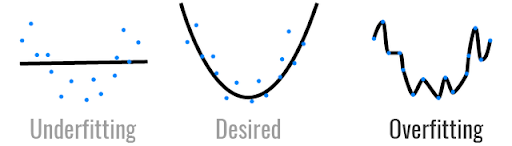
\includegraphics[width=\textwidth]{fitting-problem.png}
    \caption{Fitting Problems \cite{overfitting}}
    \label{fig:fittingProblems}
\end{figure}


\begin{figure}[ht]
    \centering
    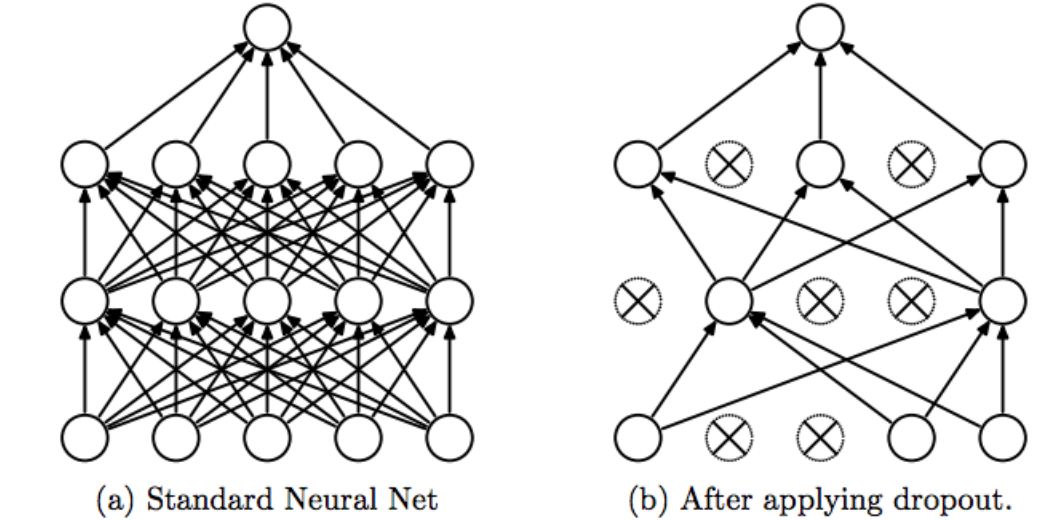
\includegraphics[width=\textwidth]{dropout.png}
    \caption{Dropout Layer \cite{dropout}}
    \label{fig:dropoutLayer}
\end{figure}
\section{Tensorflow and Python}
There are a few machine learning platforms that can help us to create our neural network. I decided to use Tensorflow because it is popular and has a big community to help. It also is built with keras which allows you to create these models from a High Level. Tensor flow also has C++ bindings that takes use of the GPU for the matrix which is far more efficient than using a normal CPU and so is quicker for handling large data-sets.

Tensorflow is mainly meant to be used in python as python is the main language for Data Science. This proved to be a problem initially as I did not know python. Although Tensorflow also provides a JavaScript library\footnote{https://www.tensorflow.org/js}, I chose to use the python version as the JavaScript library did not provide all the functionality of the main python library. It also allowed me to use Jupyter Notebook (discussed in section \ref{jupyterNotebook}) which provided a really platform to experiment with the machine learning model.

\begin{figure}[ht]
    \centering
    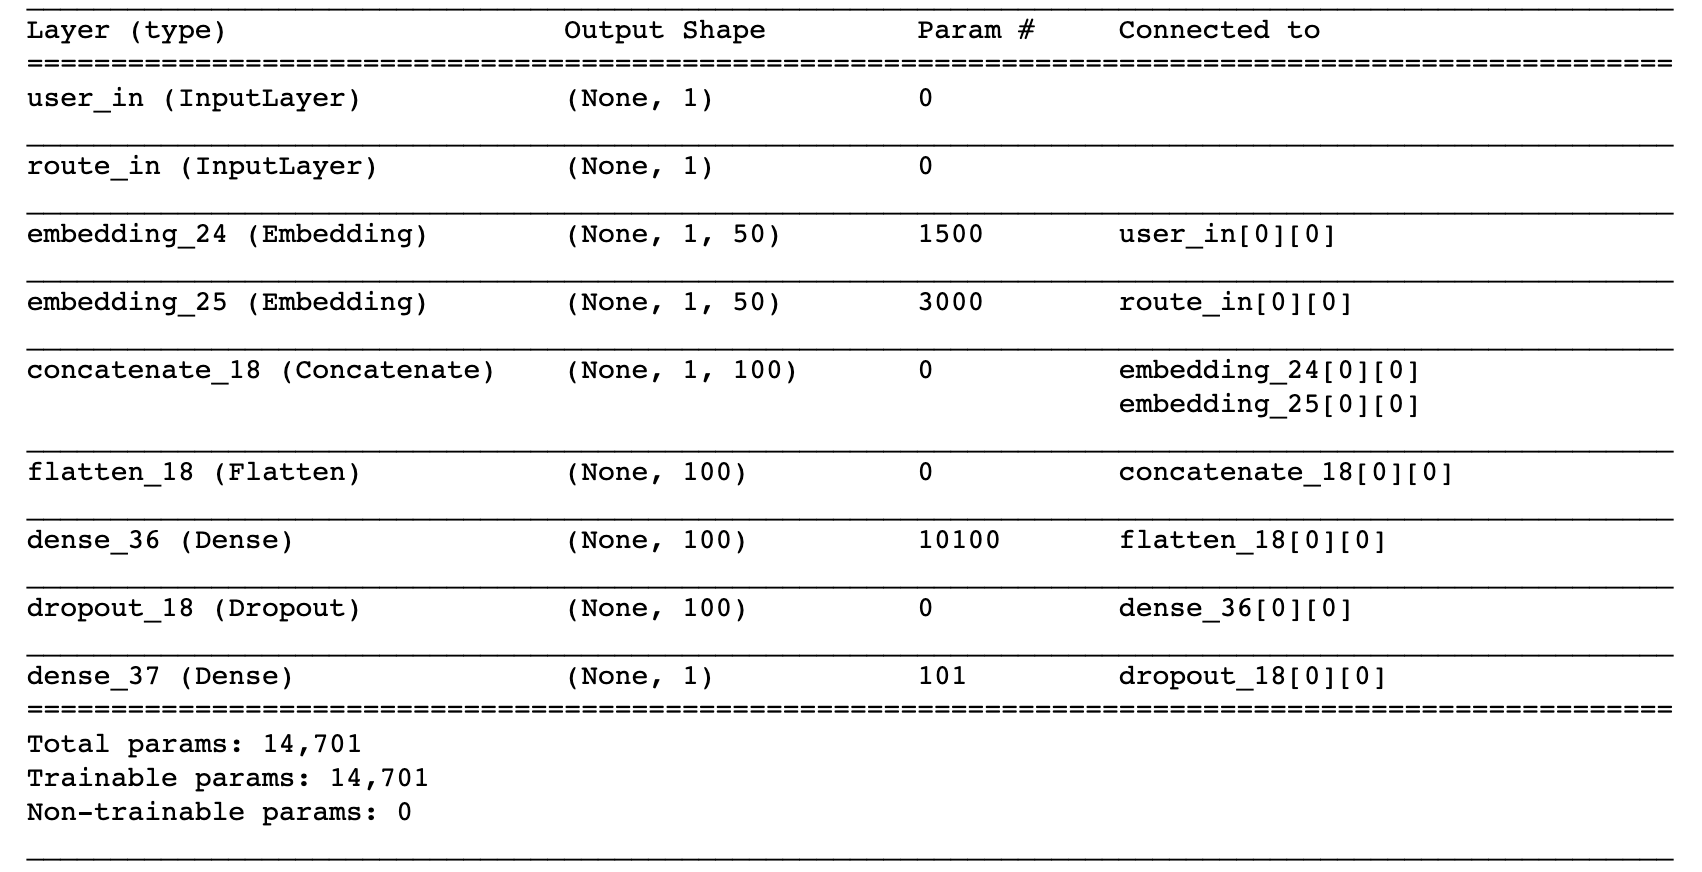
\includegraphics[width=\textwidth]{neural-net-summary.png}
    \caption{Summary of Neural Network}
    \label{fig:neuralNetworkSummary}
\end{figure}

\subsection{Jupyter Notebook} \label{jupyterNotebook}
Jupyter Notebook\footnote{https://jupyter.org/} that allows creating and running notebooks via a web application. These documents can contain both Markup text and more importantly code that is exists in cells on the document. The document allows you to easily share any code with others easily as it make's it straightforward to document. With it's use of cells, you can rerun individual blocks of code with running the entire document, making it easy to develop and iterate through different versions as you improve.
\begin{figure}[ht]
    \centering
    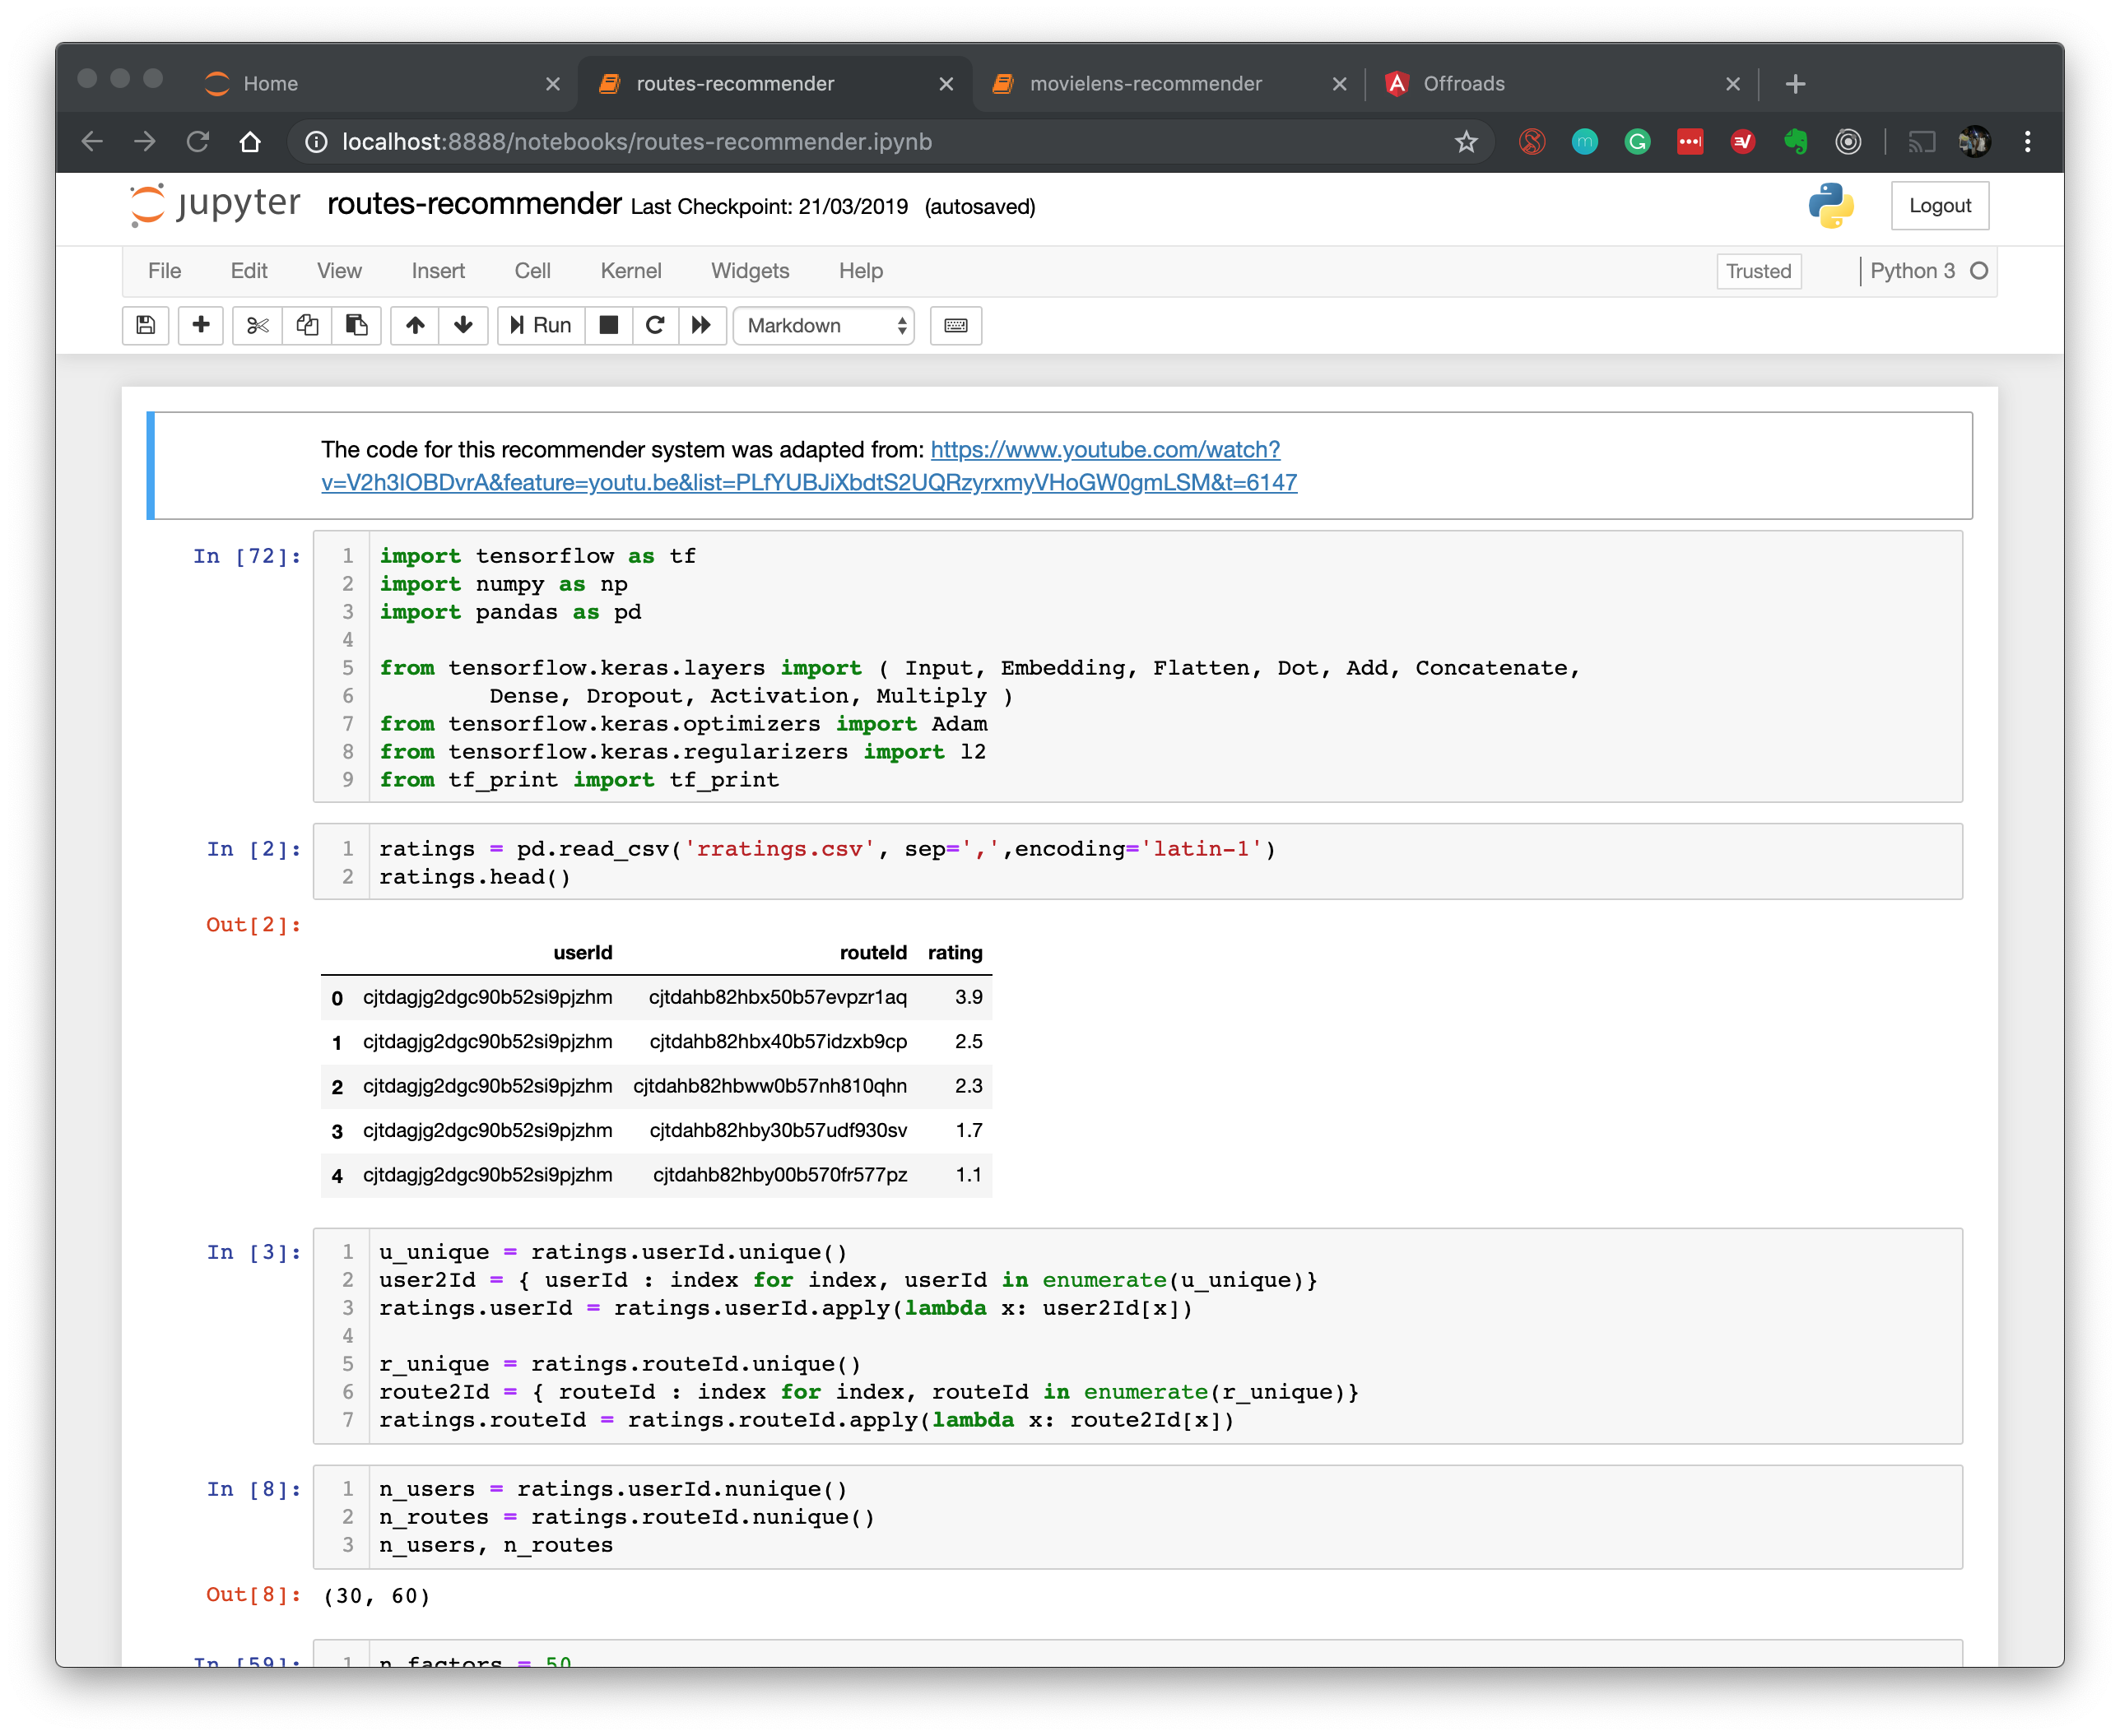
\includegraphics[width=\textwidth]{jupyter-notebook.png}
    \caption{Jupyter Notebook}
    \label{fig:JupyterNotebook}
\end{figure}

